\documentclass[12pt]{article}
\usepackage{sbc-template}
\usepackage[utf8]{inputenc}
\usepackage[T1]{fontenc}
\usepackage[brazil]{babel}
\usepackage{footnote}
\usepackage{adjustbox}


\usepackage{setspace}
\usepackage{graphicx,url}
\usepackage{multirow}
\usepackage{color,colortbl,xcolor}
\usepackage{scalefnt}
\usepackage{xspace}

\RequirePackage{hyperref}

\def\thr{\textit{throughpt}\xspace}
\def\fw{\textit{forwarding}\xspace}
\def\sw{\textit{software}\xspace}

%\sloppy

\title{Impacto da programabilidade no plano de dados em SmartNIC}

\author{Ronaldo Canofre M. dos Santos, Arthur F. Lorenzon,\\ Fabio D. Rossi, Marcelo C. Luizelli}

\address{Programa de Pós-Graduação em Engenharia de Software (PPGES)
    \\Universidade Federal do Pampa (UNIPAMPA)\\ 
    \\Instituto Federal Farroupilha (IFFAR)
    Alegrete – RS – Brasil
    \email{\{canofre, arthurlorenzon, marceloluizelli\}@unipampa.edu.br}
    \email{fabio.rossi@iffarroupilha.edu.br}
}
\linespread{0.98}

\begin{document} 
\maketitle

%%%%%%%%%%%%%%%%%%%%%%%%%%%%%%%%%%%%%%%%%%%%%%%%%%%%%%%%%%%%%%%%
\begin{resumo}
A programabilidade no plano de dados é um novo paradigma que através da linguagem P4, proporciona uma utilização mais eficiente dos dispositivos, sendo as SmartNICs disponíveis atualmente, um fator importante para sua adoção, devido a possibilidade de utilização em um ambiente real. No entanto, existem custos e limitações atreladas a este conjunto que requerem uma certa atenção. Neste trabalho é realizada avaliação utilizando um conjunto específico de configurações a fim de quantificar as limitações de desempenho existentes ainda não avaliadas. Os resultados mostram que a taxa de encaminhamento de pacotes pode alcançar uma degradação superior a 50\%.
\end{resumo}

%O trabalho investiga o impacto da programabilidade (utilizando P4) na SmartNIC NFP4000. Especificamente, o foco é direcionado para a taxa final de encaminhamento de pacotes. O contexto é relacionado com a ERRC e o tema é interessante, sobretudo considerando que diversos artigos atuais ignoram tal métrica e análise. Parabéns pela escolha do tema.


\section{Introdução} \label{sec:intro}
%%%%%%%%%%%%%%%%%%%%%%%%%%%%%%%%%%%%%%%%%%%%%%%%%%%%%%%%%%%%%%%%

A programabilidade de rede surgiu como parte da busca de novos paradigmas para gerência de redes \cite{arquitetura_programavel_18}, se tornando uma alternativa a rigidez empregada  atualmente na atualização dos dispositivos de rede, buscando mais flexibilidade, escalabilidade e controle, obtendo melhor aproveitamento atrelado a um menor custo \cite{revolucao_redes_p4_18}. A sua utilização já vem sendo abordada em trabalhos realizados nas últimas duas ou três décadas, tais como redes ativas, redes ATM programáveis e em propostas para controle e separação do plano de dados, como NCP e RCP \cite{sdn_survey_15} e mais recentemente a arquitetura SDN (\textit{Software Defined Networking}).

A ideia de tornar o  plano de dados programável foi apresentada em 2014 por \cite{p4_14}, como uma alternativa às limitações apresentadas pelos controladores das redes SDN, viabilizando uma opção mais simples, independente de protocolo e limitação de cabeçalhos pré-definidos, através da utilização de uma linguagem de alto nível denominada P4 (\textit{Programming  Protocol-independent  Packet  Processors}). Desde então, trabalhos baseados na programabilidade dos planos de dados vem sendo desenvolvidos, abordando inúmeros e distintos objetivos, no entanto, pouco se aborda sobre o impacto dessa programabilidade na capacidade de encaminhamento ou \textit{forwarding rate}.


Uma das possíveis causas para esta situação pode ser relacionada ao desenvolvimento e realização de testes em ambientes virtuais, possibilitando assim a ampliação de recursos, o que não se torna possível quando aplicada sobre dispositivos programáveis como interfaces SmartNIC ou NetFPGA. Assim, este trabalho busca realizar uma análise do impacto do uso de programas P4 sobre interfaces Agilio CX da Netronome, desenvolvidas com a arquitetura NFP4000 a fim de demonstrar os efeitos do aumento de processamento na programação voltada para o plano de dados sobre o \textit{forwarding rate}.

%Uma das possíveis causas para esta situação pode ser relacionada com o ambiente virtual geralmente utilizado para o desenvolvimento e realização de testes e a possibilidade de ampliação de recursos existentes. No entanto, quando aplicada sobre dispositivos programáveis como interfaces SmartNIC ou NetFPGA, a ampliação de recursos não se apresenta como uma possibilidade. Assim, este trabalho busca realizar uma análise do impacto do uso de programas P4 sobre interfaces Agilio CX da Netronome, desenvolvidas com a arquitetura NFP4000 a fim de demonstrar os efeitos do aumento de processamento na programação voltada para o plano de dados sobre o \textit{forwarding rate}.

O restante deste trabalho está organizado da seguinte forma. Apresenta-se na Seção \ref{sec:smartnic} a arquitetura da interface de rede utilizada, enquanto que na Seção \ref{sec:tr}, discute-se os trabalhos relacionados. Na Seção \ref{sec:implementacao}, apresenta-se a implementação, a metodologia empregada e o ambiente de avaliação. Os resultados obtidos são apresentados na Seção \ref{sec:resultados} e, por fim, a Seção \ref{sec:conclusoes} apresenta as considerações finais e perspectivas futuras.

\section{SmartNICs Netronome} \label{sec:smartnic}
%%%%%%%%%%%%%%%%%%%%%%%%%%%%%%%%%%%%%%%%%%%%%%%%%%%%%%%%%%%%%%%%

As SmartNICs ou NICs inteligentes, podem se consideradas interfaces completamente programáveis, com um processamento paralelo e multi core baseado em uma abordagem SoC (\textit{Systen-on-chip}), a qual combina uma ou mais CPUs com as funções padrões da NIC \cite{intro_snic_19}.  A SmartNIC NFP4000 \cite{nfp4000_16} utilizada, apresenta uma arquitetura modular composta por ilhas, tais como de memórias e de unidades de processamento, vide figura \ref{fig:nfp_arquitetura}. Estas unidades são máquinas de 32 \textit{bits} denominadas FPCs (\textit{Flow Processing Cores}), com  espaços distintos para armazenamento de dados e instruções, permitindo que cada unidade execute um conjunto diferenciado de ações.

\begin{figure}[!t]
\centering
\resizebox{10cm}{!}{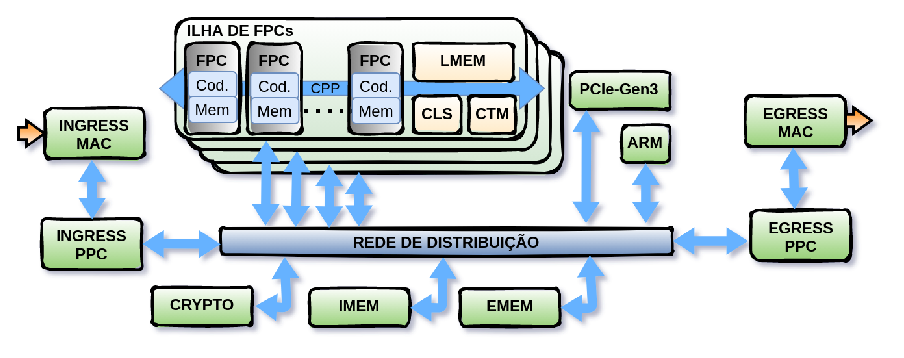
\includegraphics{img/nfp_arquitetura}}
%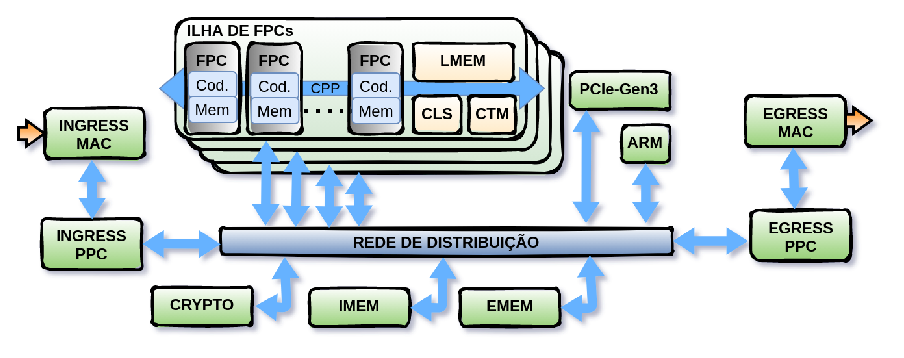
\includegraphics[scale=1.2]{img/nfp_arquitetura}
\caption{Arquitetura NFP4000}
\label{fig:nfp_arquitetura}
\end{figure}

As FPCs contam também com 8 \textit{threads} que atuam sobre o mesmo código e memória local, trocando informações entre os componentes através de um barramento denominado CPP (\textit{command-push-pull}). Cada FPC é composta ainda por uma memória local com 1024 palavas de 32 \textit{bits} e três conjuntos de registradores, sendo 256 de propósito geral, divididos entre as 8 \textit{threads}, 512 de transferência, utilizados para trafegar dados no barramento CPP e 128 do tipo \textit{next-neighbor}, utilizados na comunicação com FPCs vizinhas na mesma ilha. A interface contém ainda 5 ilhas de processamento compostas por 12 FPCs e uma memória local (LMEM) de 4KB, podendo possuir ainda outros dois tipos de memória: CLS de 64KB, para dados necessários à maioria dos pacotes e CTM de 256 KB, para cabeçalhos de pacotes e coordenação entre FPCs e outros sub-sistemas. 

Externamente as ilhas de processamento, cada interface possui ainda mais duas memórias: IMEM de 4MB, destinada ao corpo dos pacotes e compartilhamento de tabelas médias (2 por interface) e (EMEM) de 3MB + DRAM, para compartilhamento de grandes tabelas (3 por \textit{chip}) \cite{nfp4000_20}. A programação destas interfaces pode ser realizada através de linguagens de alto nível como P4 e Micro-C através de um compilador proprietário, apresentando no entanto algumas restrições e diferenças comportamentais com relação ao P4 modelo. A linguagem Micro-C consiste em um subconjunto do Standard C, principalmente devido a limitações relacionadas aos tipos de dados suportados, funções e cabeçalhos de biblioteca padrão.

\section{Trabalhos relacionados} \label{sec:tr}
%%%%%%%%%%%%%%%%%%%%%%%%%%%%%%%%%%%%%%%%%%%%%%%%%%%%%%%%%%%%%%%%

Esforços consideráveis voltados ao uso eficiente de aplicativos em SmartNICS tem sido realizados, tais como DAIET \cite{daiet_17} e Clara \cite{clara_20}, que assim como a grande maioria dos trabalhos, se destinam a avaliação do descarregamento da aplicação no plano de dados, não levando em consideração as limitações atuais das SmartNICs, deixando de lado a avaliação do impacto causado pelas estruturas e pelo processamento realizado. Por outro lado, alguns trabalhos tem focado na análise das estruturas e componentes de programas P4 e no impacto sobre o desempenho do processamento em interfaces inteligentes. 

Em \cite{harkous_19}, é apresentada uma avaliação do impacto na latência de processamento de pacotes realizada em diferentes programas P4, realizando o aumento gradativo da complexidade através da inclusão de alguns blocos como analisador e controle, buscando identificar as variáveis mais influentes para prever a latência do pacote. Já em \cite{pablo_21}, é realizada uma análise do \thr e latência, através da elevação quantidade das métricas utilizadas, analisando o volume de operações em registradores, de acessos em tabelas de fluxo, de recirculação de pacotes, de funções de criptografia e de operações aritméticas.

No entanto, tais trabalhos não ponderam as questões referentes a adição de campos mais simples, como cabeçalhos adicionais ou personalizados, não sendo também realizadas avaliações relativas a utilização de componentes externos, como o uso de módulos em Micro-C ou análises referentes ao controle de concorrência e o impacto trazido com seu uso. Ademais, tais trabalhos não consideram a limitação de utilização de processadores, até o momento necessária para obtenção de uma corretude na computação de valores em todos os pacotes, os quais implicam na diminuição do \thr. Assim sendo, este trabalho busca contribuir com as avaliações do impacto do P4 em SmartNICs através da análise dos pontos supracitados.

\section{Implementação e metodologia} \label{sec:implementacao}
%%%%%%%%%%%%%%%%%%%%%%%%%%%%%%%%%%%%%%%%%%%%%%%%%%%%%%%%%%%%%%%%
%Nesta seção são abordadas as implementações realizadas, explanando sobre os casos de testes realizado, abordando ainda a metodologia e o ambiente de testes.

Como ponto de partida, utilizou-se o código de encaminhamento de pacotes disponibilizado pelo P4.org (caso 1\footnote{https://github.com/p4lang/tutorials/tree/master/exercises/basic}), a partir do qual foram realizadas inclusões de estruturas e funcionalidades de forma complementar ao caso anterior, sendo  analisando o impacto sobre a quantidade de pacotes encaminhados a cada nova alteração. Para o caso 2, foi adicionado um cabeçalho UDP juntamente com sua inicialização, seguido da adição de um cabeçalho personalizado denominado APF compostos de 4 campos de 32 \textit{bits} e um campo de 2 \textit{bits} (caso 3) e por fim de um cabeçalho de metadados contento dois campos de 64 \textit{bits} com registros de \textit{timestamp} de ingresso no dispositivo e atual (caso 4), todos sem utilização no processamento do plano de dados. 

Posteriormente foi atribuído ao cabeçalho APF a transposição de informações entre os estágios do processamento (caso 5), seguido da recuperação do tamanho do pacote, cálculo da latência e seu respectivo armazenamento em um registrador de 32 \textit{bits} (caso 6). Devido as limitações de processamentos apresentadas pela interface da Netronome ao se realizar uma correta computação de latência para o grande volume de dados enviados, foi adicionada a implementação de um módulo em Micro-C, responsável pelo cálculo da média entre as métricas disponíveis (caso 7).% sendo posteriormente adico um contador de pacotes (caso 8) % é no caso 8 mais vai junto com mutex

A partir desta programação, buscando também avaliar o impacto das metodologias disponíveis para o tratamento do paralelismo, foi adicionado um contador de pacotes e realizada uma avaliação com o uso do mecanismos de controle de concorrência mutex (caso 8) e semáforo (caso 11), sendo o primeiro disponibilizado pelas bibliotecas da Netronome e segundo programado em Micro-C. Considerando que nestas avaliações é realizado o bloqueio da execução para todos os pacotes, foram também analisadas reduções na sua utilização, realizando a aplicação dos bloqueios a cada 5 e 100 pacotes, tanto para mutex (casos 9 e 10) como para semáforo (casos 12 e 13).% para mutex (caso 9), semáforo (caso 12) e a com a aplicação do bloqueio a cada 100 pacotes também para mutex (caso 10), semáforo (caso 13).  

O ambiente de desenvolvimento consiste em dois servidores com processador AMD Ryzen 7 3800X com 8 cores e 24GB de RAM, com interfaces Netronome SmartNIC Agilio CX 10 Gbit/s, sendo um deles utilizado para carregamento dos programas P4, atuando como comutador, e o outro utilizado como gerador de tráfego. Foi utilizado o gerador de pacotes da Netronome, através do gerador de trafego DPDK\footnote{https://www.dpdk.org/} disponibilizado pelo MoonGen \cite{mg_14}. Foram enviados pacotes IPv4 de 64B com endereços de origem e destino fixos por intervalos de 10 segundos, sendo cada resultado obtido através de uma média simples de três execuções. Foram também aplicadas reduções para limitação da quantidade de processadores utilizados, reduzindo a capacidade de encaminhamento da interface, a qual gira em torno de 10 Gbps para cerca de 2.5 Gbps.

\section{Resultados} \label{sec:resultados}
%%%%%%%%%%%%%%%%%%%%%%%%%%%%%%%%%%%%%%%%%%%%%%%%%%%%%%%%%%%%%%%%

A figura \ref{fig:casos_grafico} apresenta os resultados dos casos 1 à 8, sendo possível perceber a existência do impacto na taxa de encaminhamento em cada caso, mesmo que mínimo. No caso 2 à 4 é possível perceber uma leve degradação a cada  inclusão de um novo cabeçalho, resultando em um o impacto de 6.34\% somente com a adição de três novos cabeçalho, demonstrando a existência de uma degradação relacionada a quantidade destes campos. Nos casos 5 e 6 são apresentadas as maiores variações observadas, oriundas da inclusão de operações no plano de dados. No caso 5, o custo da utilização do cabeçalho APF é de 15.17\% em relação ao caso anterior, elevando-se para 20.55\% quando comparado com o processamento inicial.

\begin{figure}[!htb]
\centering
\resizebox{9cm}{!}{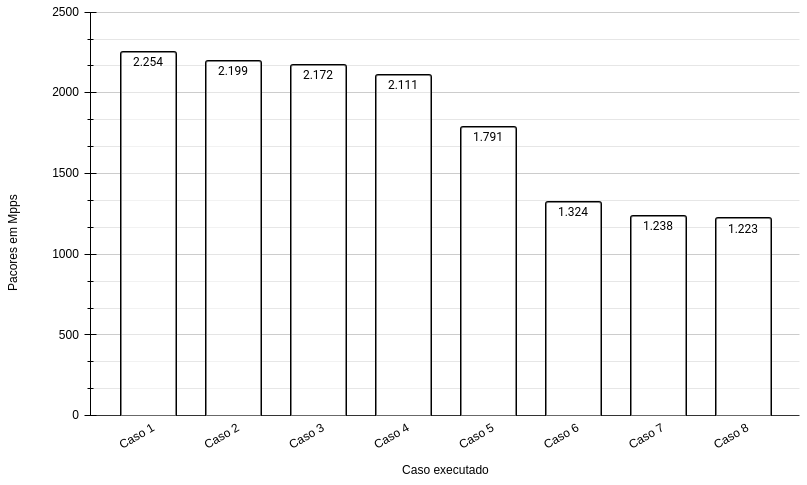
\includegraphics{img/casos_grafico}}
\caption{Quantidade de pacotes por caso executado.}
\label{fig:casos_grafico}
\end{figure}

No caso 6, o impacto apresentado em realação a execução anterior é  mais significativo, cerca de 26\%, elevando-se para cerca de 41\% em relação ao processamento inicial, praticamente o dobro do impacto anterior (20.55\%), demonstrando a existência de degradação atrelada ao processamento empregado, visto que no caso 5 somente ocorre a inicialização de campos no cabeçalho APF e no caso 6 são realizados além da inicialização de campos com cálculos, o armazenamento dos valores em registradores internos do plano de dados. Já nos casos seguintes, onde ocorre a inclusão do módulo em Micro-C (caso 7) e a utilização de um controle de concorrência com mutex (caso 8), é possível verificar que o impacto com relação aos casos anteriores não é extremamente elevado, gerando no entanto um custo acumulado de mais de 45\% na quantidade de pacotes encaminhando ao final de todos os incrementos de processamento realizados até o caso 8.

A tabela \ref{tab:bloqueios} apresenta os resultados dos testes de controle de concorrência implementados com mutex e semáforo, sendo possível avaliar que são muito próximos os impactos causados por ambos os casos (8 e 11) sobre o processamento, onde o uso do semáforo apresenta um custo de apenas 0.6\% a mais que o uso do mutex, em comparação ao processamento inicial. No entanto, ao se implementar uma redução no uso dos bloqueios, é possível avaliar que em ambos os métodos utilizados ocorre um acréscimo no custo de processamento, resultando em uma degradação superior a 50\% em comparação com o processamento inicial, ao contrário do esperado. Por fim, a aplicação do bloqueio de concorrência em um intervalo maior de pacotes (casos 10 e 13) não resulta em uma diferença significativa da quantidade de pacotes encaminhados, mantendo resultados idênticos ou muito próximos. 

\begin{table}[!htb]
    \centering
    \caption{Encaminhamento de pacotes por bloqueio implementado.}
    \label{tab:bloqueios}
    \begin{tabular}{| l | c | l |} \hline
        Caso    &Taxa de encaminhamento & Descrição\\ \hline
        Caso 8  &1.223 Mpps & mutex\\ \hline
        Caso 9  &1.101 Mpps & mutex a cada 5 pacotes\\ \hline
        Caso 10  &1.102 Mpps & mutex a cada 100 pacotes\\ \hline
        Caso 11  &1.210 Mpps & semáforo \\ \hline
        Caso 12  &1.005 Mpps & semáforo a cada 5 pacotes\\ \hline
        Caso 13  &1.005 Mpps & semáforo a cada 100 pacotes\\ \hline
    \end{tabular}
\end{table}


\section{Conclusão} \label{sec:conclusoes}
%%%%%%%%%%%%%%%%%%%%%%%%%%%%%%%%%%%%%%%%%%%%%%%%%%%%%%%%%%%%%%%%

Neste trabalho analisou-se o impacto da adição de componentes em um programa P4 sobre a taxa de encaminhamento de pacotes em interfaces SmarNIC. Através dos testes realizados foi possível observar a ocorrência de degradação em todos os casos, sendo mais evidenciada na inclusão de processamento no plano de dados, ocorrendo em uma escala inferior quando da adição de cabeçalhos e adição de módulos externos.  
%Ainda, relacionado ao controle de concorrência, foi possível verificar que o método utilizado não aplica uma grande distinção no desempenho e que no cenário adotado, a alteração do intervalo ao qual os bloqueios são aplicada também não interferem nos resultados.
Relacionado as avaliações de controle de concorrência, foi possível avaliar que a utilização de mutex ou semáforo resultam em um impacto muito próximo, sendo mais prejudicial a aplicação de bloqueios parciais em ambos os controles.

Os resultados obtidos servirão também como parâmetro para comparações e análise, no desenvolvimento de um protótipo de monitoramento e detecção preditiva de anomalias sob o mesmo ambiente utilizado. No entanto, algumas questões podem ainda ser avaliadas em trabalhos futuros, tais como a possibilidade dos resultados estarem relacionados como a interface utilizada, sendo a comparação com outras NICs inteligentes uma avaliação a ser realizada. Outro ponto a ser analisado futuramente, denota sobre a existência ou não da estabilidade na degradação. 

% Posteriormente, almeja-se realizar um aprofundamento sobre o funcionamento da interface, a fim de verificar a viabilidade de distribuir o processamento entre as FPCs, melhorando o desempenho.

\section*{Agradecimentos} \label{sec:ack}
Este trabalho foi parcialmente financiado por: 
Fundação de Amparo à Pesquisa do Estado de São Paulo (FAPESP) -- 2018/23092-1, 2020/05183-0, 2020/05115-4; Fundação de Amparo à Pesquisa do Estado do Rio Grande do Sul (FAPERGS) -- 19/2551-0001266-7, 19/2551-0001224-1, 19/2551-0001689-1, 21/2551-0000688-9; e pelo Conselho Nacional de Desenvolvimento Científico e Tecnológico (CNPq) -- 427814/2018-9.


%\singlespacing
%\begin{spacing}{.1}
\bibliographystyle{sbc}
\bibliography{bibliografia}
%\end{spacing}
\end{document}